\documentclass[conference]{IEEEtran}
\IEEEoverridecommandlockouts
% The preceding line is only needed to identify funding in the first footnote. If that is unneeded, please comment it out.
\usepackage{cite}
\usepackage{amsmath,amssymb,amsfonts}
\usepackage{algorithmic}
\usepackage{graphicx}
\usepackage{textcomp}
\usepackage{xcolor}
\usepackage{caption}
\usepackage{subcaption}

\def\BibTeX{{\rm B\kern-.05em{\sc i\kern-.025em b}\kern-.08em
    T\kern-.1667em\lower.7ex\hbox{E}\kern-.125emX}}
\begin{document}

\title{Semiconductor Materials for\\Ultra High Frequency Transistors
    \thanks{University of Washington Bothell}
}

\author{\IEEEauthorblockN{Pongpak Techagumthorn}
    \IEEEauthorblockA{\textit{Physical Sciences Division} \\
        \textit{Univ. of Washington Bothell}\\
        Bothell, USA \\
        pongpakt@uw.edu}
}

\maketitle

\begin{abstract}
    Our modern day world is ever more reliant on connected devices. Inside every one of these devices there is a microprocessor
    inside. Currently the overwhelming majority of these microprocessors are constructed from silicon. As technology progresses
    we require ever faster processors. We are at a point now where we are reaching the limits of what silicon can provide. Scientists
    and engineers have turned to new semiconductor materials to overcome these limits. One such semiconductor material is Indium
    Gallium Phosphide (InGaP).

    This project aims to compare ultra-high frequency (0.3 - 3 GHz) characteristics of Silicon and Indium Gallium Phosphide in an
    LTSpice environment. For the transistor model we will be using the hybrid-$pi$ equivalent circuit transistor model.
    On the silicon side of things we will be simulating the general purpose 2N3904 NPN transistor. For the
    InGaP transistor we will be looking at the ERA-50SM+ device. Before simulating a complex device such as the ERA-50SM+ we started
    with small scale common emitter and common collector amplifier circuits. After running or small scale simulations we realized
    that the hybrid-$pi$ model was inadequate for our tests. Due to time constraints we were not able to come to a consensus
    for our research question.
\end{abstract}

\begin{IEEEkeywords}
    Transistors, Semiconductors, Silicon, InGaP, LTSpice
\end{IEEEkeywords}

\section{Introduction}

\subsection{Background}

\IEEEPARstart{E}{verywhere} we look more and more of our devices are being connected to the internet, from our phones
and computers to our cars and even our kitchen appliances. These so called "smart devices" are made
to accomplish a myriad of tasks but share one thing in common, they all have some sort of microprocessor
inside them to control what they do. Looking back at the history of microprocessors, and the transistors
that provided their building blocks, the prevailing semiconductor material used within these devices has
been silicon. The earliest transistors were constructed from germanium due to the ease of production at
a high purity monocrystalline form \cite{Early2001}. In the early 1950s a way to produce monocrystalline silicon was
developed and since then the industry has largely switched over to silicon. From the onset of transistor technology
scientists knew that silicon would be superior to germanium for transistors \cite{Jenkins2005}. The larger band gap in
silicon made silicon-based transistors more reliable and less susceptible to random noise from internal
and external sources \cite{Early2001,Jenkins2005}. The earliest, and most basic, transistors were bipolar junction transistors (BJTs).
These BJT devices consist of three semiconductor regions of alternating positive-negative-positive (PNP) or
negative-positive-negative (npn) doping, shown in fig. \cite{sze_physics_2007}. The two junctions allow small base input currents
to control much higher currents between the collector and emitter \cite{sze_physics_2007}. This allows BJTs to function
as either a swicth or an amplifier \cite{horowitz_art_2015}.

\begin{figure}[htbp]
    \centering
    \hspace*{\fill}
    \begin{subfigure}[b]{0.2\textwidth}
        \centerline{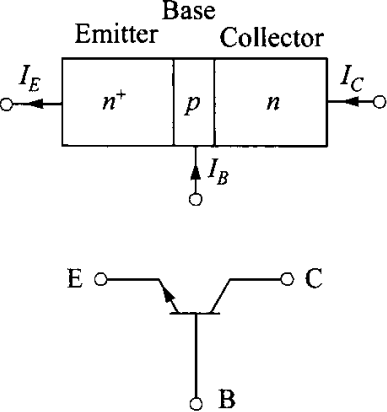
\includegraphics[width=\textwidth]{figures/NPN.png}}
        \caption{NPN}
    \end{subfigure}
    \hspace*{\fill}
    \begin{subfigure}[b]{0.2\textwidth}
        \centerline{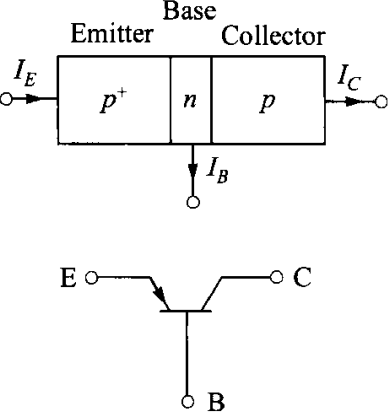
\includegraphics[width=\textwidth]{figures/PNP.png}}
        \caption{PNP}
    \end{subfigure}
    \hspace*{\fill}
    \caption{Simplified internal construction, nomenclatures, and symbols of (a) NPN and (b) PNP transistors
    \\ Source: Adapted from \cite{sze_physics_2007}}
    \label{fig:transistor-block}
\end{figure}

In the past decade we have gotten closer and closer to the limits of silicon BJTs, especially in ultra high and
extremely high frequency applications that operate in the order of 1 – 100 GHz ($10^{9}$ Hz – $10^{11}$ Hz)
\cite{Schwierz2007}. One solution that scientists and engineers have tuned to is the use of newer semiconductor
materials. These new materials have electrical properties that are more suited for ultra high (UHF) to extremely high frequency (EHF)
applications and beyond \cite{Keyes2005}. Some new semiconductor materials that have already been implemented to
address these limitations include Indium and Gallium based semiconductor materials \cite{Schwierz2007}.

\begin{figure}[htbp]
    \centerline{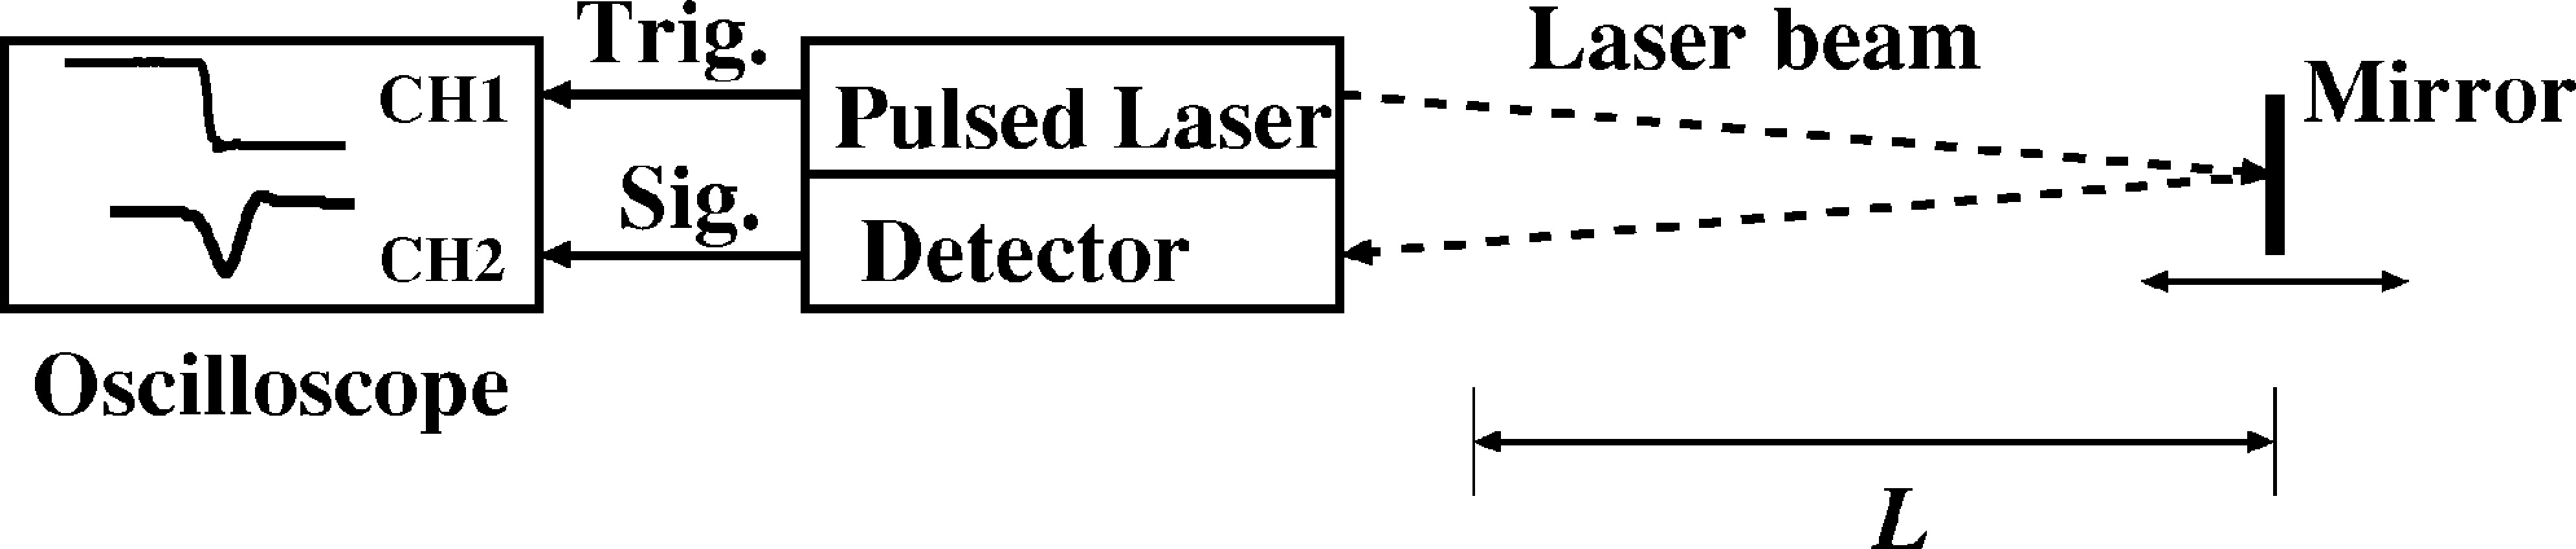
\includegraphics[width=0.5\textwidth]{figures/speed-of-light.jpeg}}
    \caption{Block diagram of the Aoki and Mitsui speed of light lab.
    The ERA-50SM+ device is part of the Pulsed Laser circuitry \\ Source: \cite{Aoki2008}}
    \label{fig:speed-of-light}
\end{figure}

An example of a device that makes use of Indium based transistors, specifically Indium Gallium Phosphide (InGaP),
is Kenichiro Aoki and Takahisa Mitsui's classic tabletop direct speed of light measurement lab \cite{Aoki2008}.The lab uses a
very high speed laser pulse and a detector to directly measure the speed of light, seen in fig. \ref{fig:speed-of-light} . Inside
the pulse circuit there is an ERA-50SM+ wide band monolithic amplifier that supports signals from DC up to 2 GHz \cite{ERA-50SM+}.
This amplifier uses a pair of NPN InGaP heterojunction bipolar transistors (HBT) in a Darlington pair, seen in fig.
\ref{fig:ERA-50SM}. HBTs function on the same principle as BJTs but instead of having the same semiconductor material at the 2 outer


\begin{figure}[htbp]
    \centerline{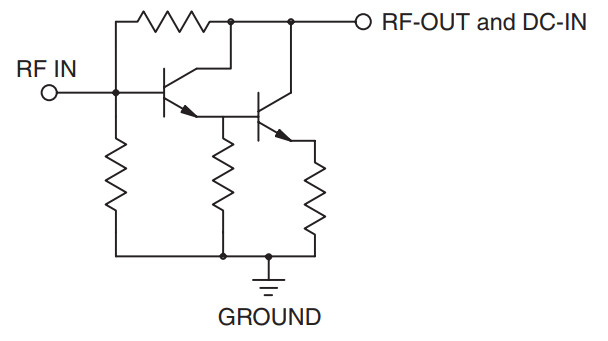
\includegraphics[width=0.3\textwidth]{figures/era50sm-schematic.png}}
    \caption{Simplified internal schematic of the ERA-50SM+ wide band monolithic amplifier \\ Source: \cite{ERA-50SM+}}
    \label{fig:ERA-50SM}
\end{figure}

Another solution that scientists and engineers use to overcome the limits of silicon BJTs is using faster switching transistor
technologies. Technologies such as  Field Effect Transistors (FET) are much better suited for these frequencies \cite{Schwierz2007}.
For this paper we choose to focus only on differing semiconductor materials in junction transistors, a superset of BJTs and HBTs,
since the ERA-50SM+ device exclusively uses this type of transistor.

\subsection{Purpose}

The goal of this project is to run simulations on InGaP HBTs and silicon BJTs and within an LTSpice environment to determine the more
suitable semiconductor material for ultra high frequency applications. Additionally we will also determine suitable applications for
each semiconductor material and the intrinsic electrical properties that make one semiconductor more suitable for ultra high frequency
applications over another.

\section{Methods}

\subsection{Evaluation Methods}

To evaluate the performance of the InGaP HBTs in comparison to standard silicon BJTs we will be simulating the ERA-50SM+ internal
circuit from fig. \ref{fig:ERA-50SM} within the manufacturer prescribed evaluation circuit, shown in fig. \ref{fig:ERA-Test-circuit}.
For the ERA-50SM+ device in fig. \ref{fig:ERA-Test-circuit} we will be constructing the internal circuitry as shown in fig. \ref{fig:ERA-50SM}
with both silicon and InGaP parameters

\begin{figure}[htbp]
    \centerline{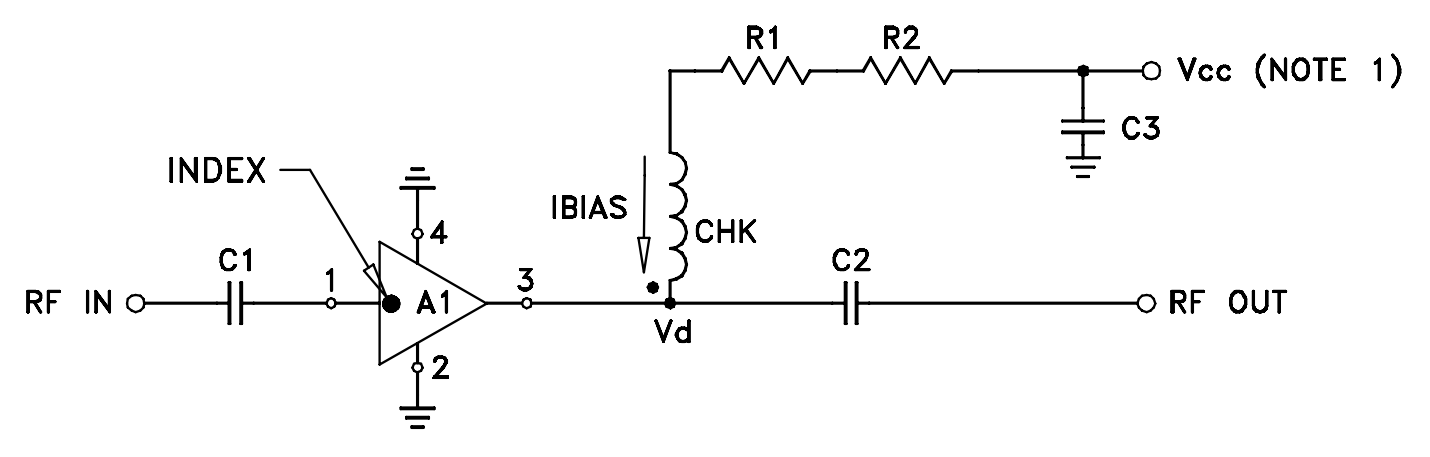
\includegraphics[width=0.5\textwidth]{figures/era-test-circuit.png}}
    \caption{ERA-50SM+ evaluation circuit as prescribed by the manufacturer \\ Source: \cite{ERA-50SM+}}
    \label{fig:ERA-Test-circuit}
\end{figure}

Before simulating the entire ERA-50SM+ device in the prescribed evaluation circuit, fig. \ref{fig:ERA-Test-circuit} we will first
simulate each type of transistor within simple circuits. We will compare the simple circuit results to manufacturer provided
performance metrics to verify that the simulated components matches expected real world performance. For the silicon BJT model we will
be simulating the 2N3904 NPN BJT with parameters from KEC Semiconductor Corp \cite{3904}. For the InGaP HBT model we will be
determining parameters from literature \cite{Oka2001,Low1999} as we do not know the specific parameters for the HBTs within the
ERA-50SM+ device.

For the simple circuit testing we will be using basic common emitter and common collector transistor amplifier circuits,
fig. \ref{fig:NPN-CE-fig} and \ref{fig:NPN-CC-fig} respectively. The common emitter amplifier configuration produces a simple
voltage amplification circuit and the common collector circuit produces a simple current amplification circuit

\begin{figure}[htbp]
    \centering
    \begin{subfigure}[b]{0.3\textwidth}
        \centerline{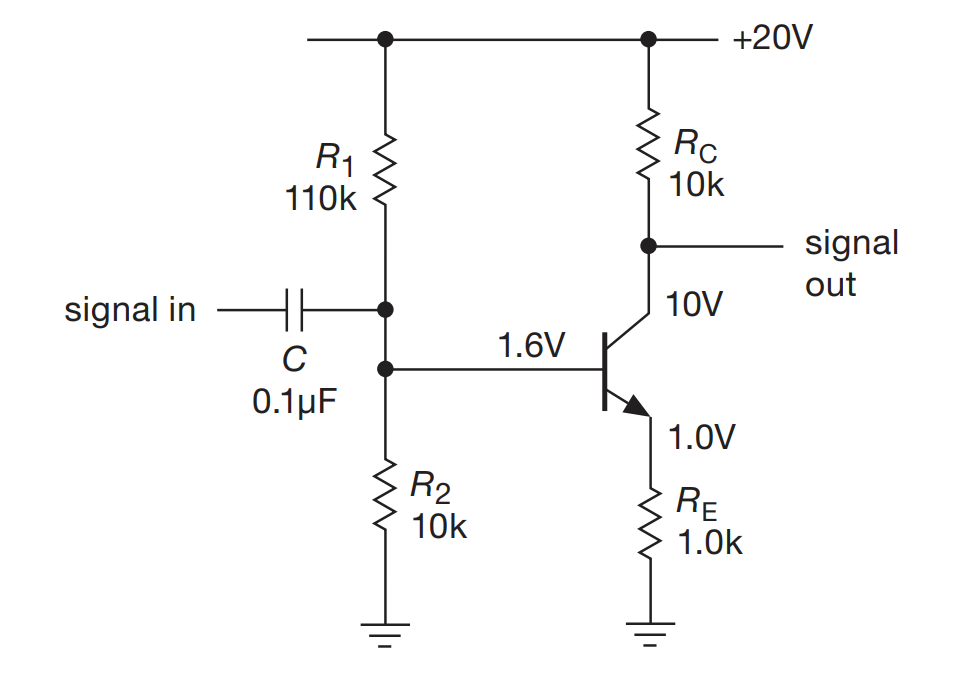
\includegraphics[width=\textwidth]{figures/NPN_CE-pic.png}}
        \caption{Common Emitter}
        \label{fig:NPN-CE-fig}
    \end{subfigure}
    \begin{subfigure}[b]{0.25\textwidth}
        \centerline{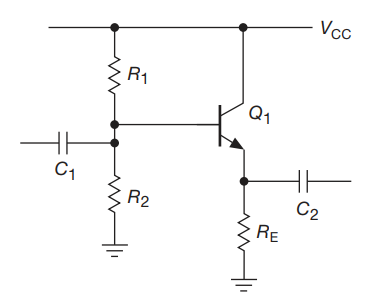
\includegraphics[width=\textwidth]{figures/NPN_CC-pic.png}}
        \caption{Common Collector}
        \label{fig:NPN-CC-fig}
    \end{subfigure}
    \caption{Simple NPN amplifier circuits \\ Source: \cite{horowitz_art_2015}}
\end{figure}

\begin{figure}[htbp]
    \centerline{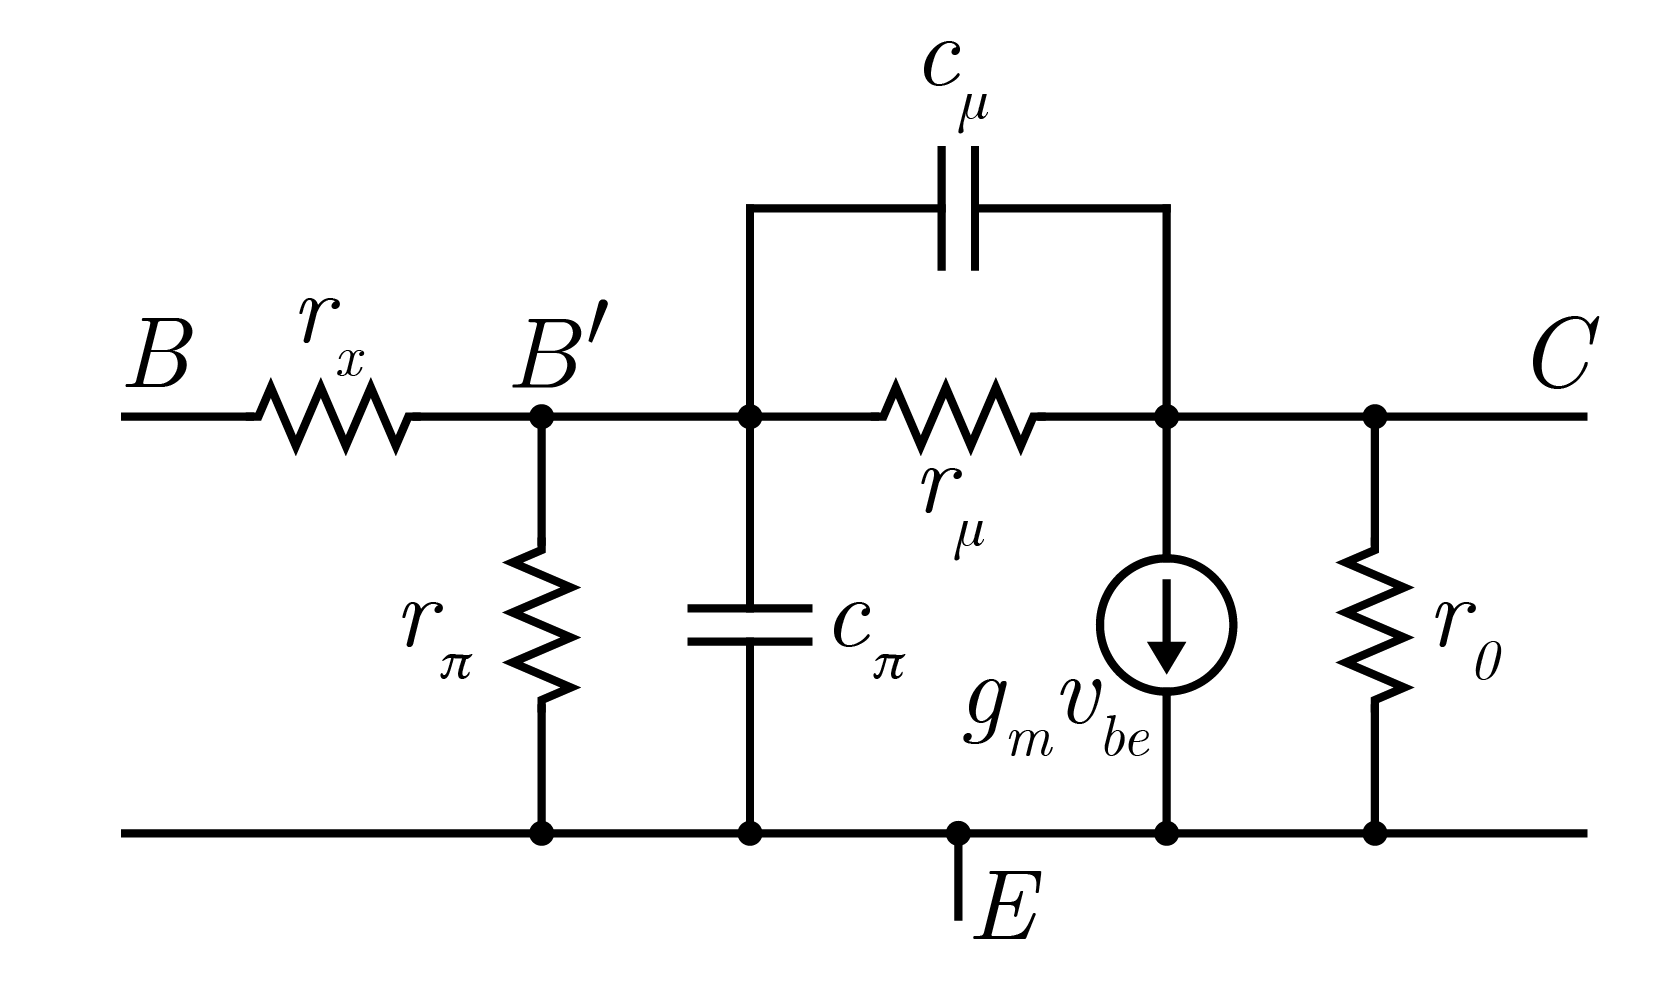
\includegraphics[width=0.4\textwidth]{figures/hybrid-pi.png}}
    \caption{Hybrid-$\pi$ equivalent circuit model for NPN transistors}
    \label{fig:hybrid-pi-model}
\end{figure}

\subsection{Hybrid-$\pi$ Model}

To model the transistor devices we will be using the hybrid-$\pi$ equivalent circuit model, shown in fig. \ref{fig:hybrid-pi-model}.
The hybrid-$\pi$ model was chosen since its parameters are easily calculated from information provided in component datasheets and
its relative accuracy in modeling junction transistor behavior across low and high frequencies \cite{Sharma1989,Malik1990}. This
model is able to function across a wide range of frequencies since it takes into account both basic parameters and parasitic
electrical properties of junction transistors \cite{Sharma1989}. The basic parameters needed for a simple hybrid-$\pi$ model are
the input resistance $r_\pi$, output resistance $r_0$, and the transconductance  $g_{m}v_{be}$ \cite{Malik1990}. These
three parameters are adequate for dc and low frequency simulations but for higher frequency simulations we need to add addition
parasitic elements. The base-emitter capacitance $c_\pi$, spreading resistance $r_x$, feedback resistance $r_\mu$, and interelectrode
capacitance $c_\mu$ compensate for high frequency effects within the stricture of the transistor \cite{Sharma1989}.

\begin{figure}[htbp]
    \centerline{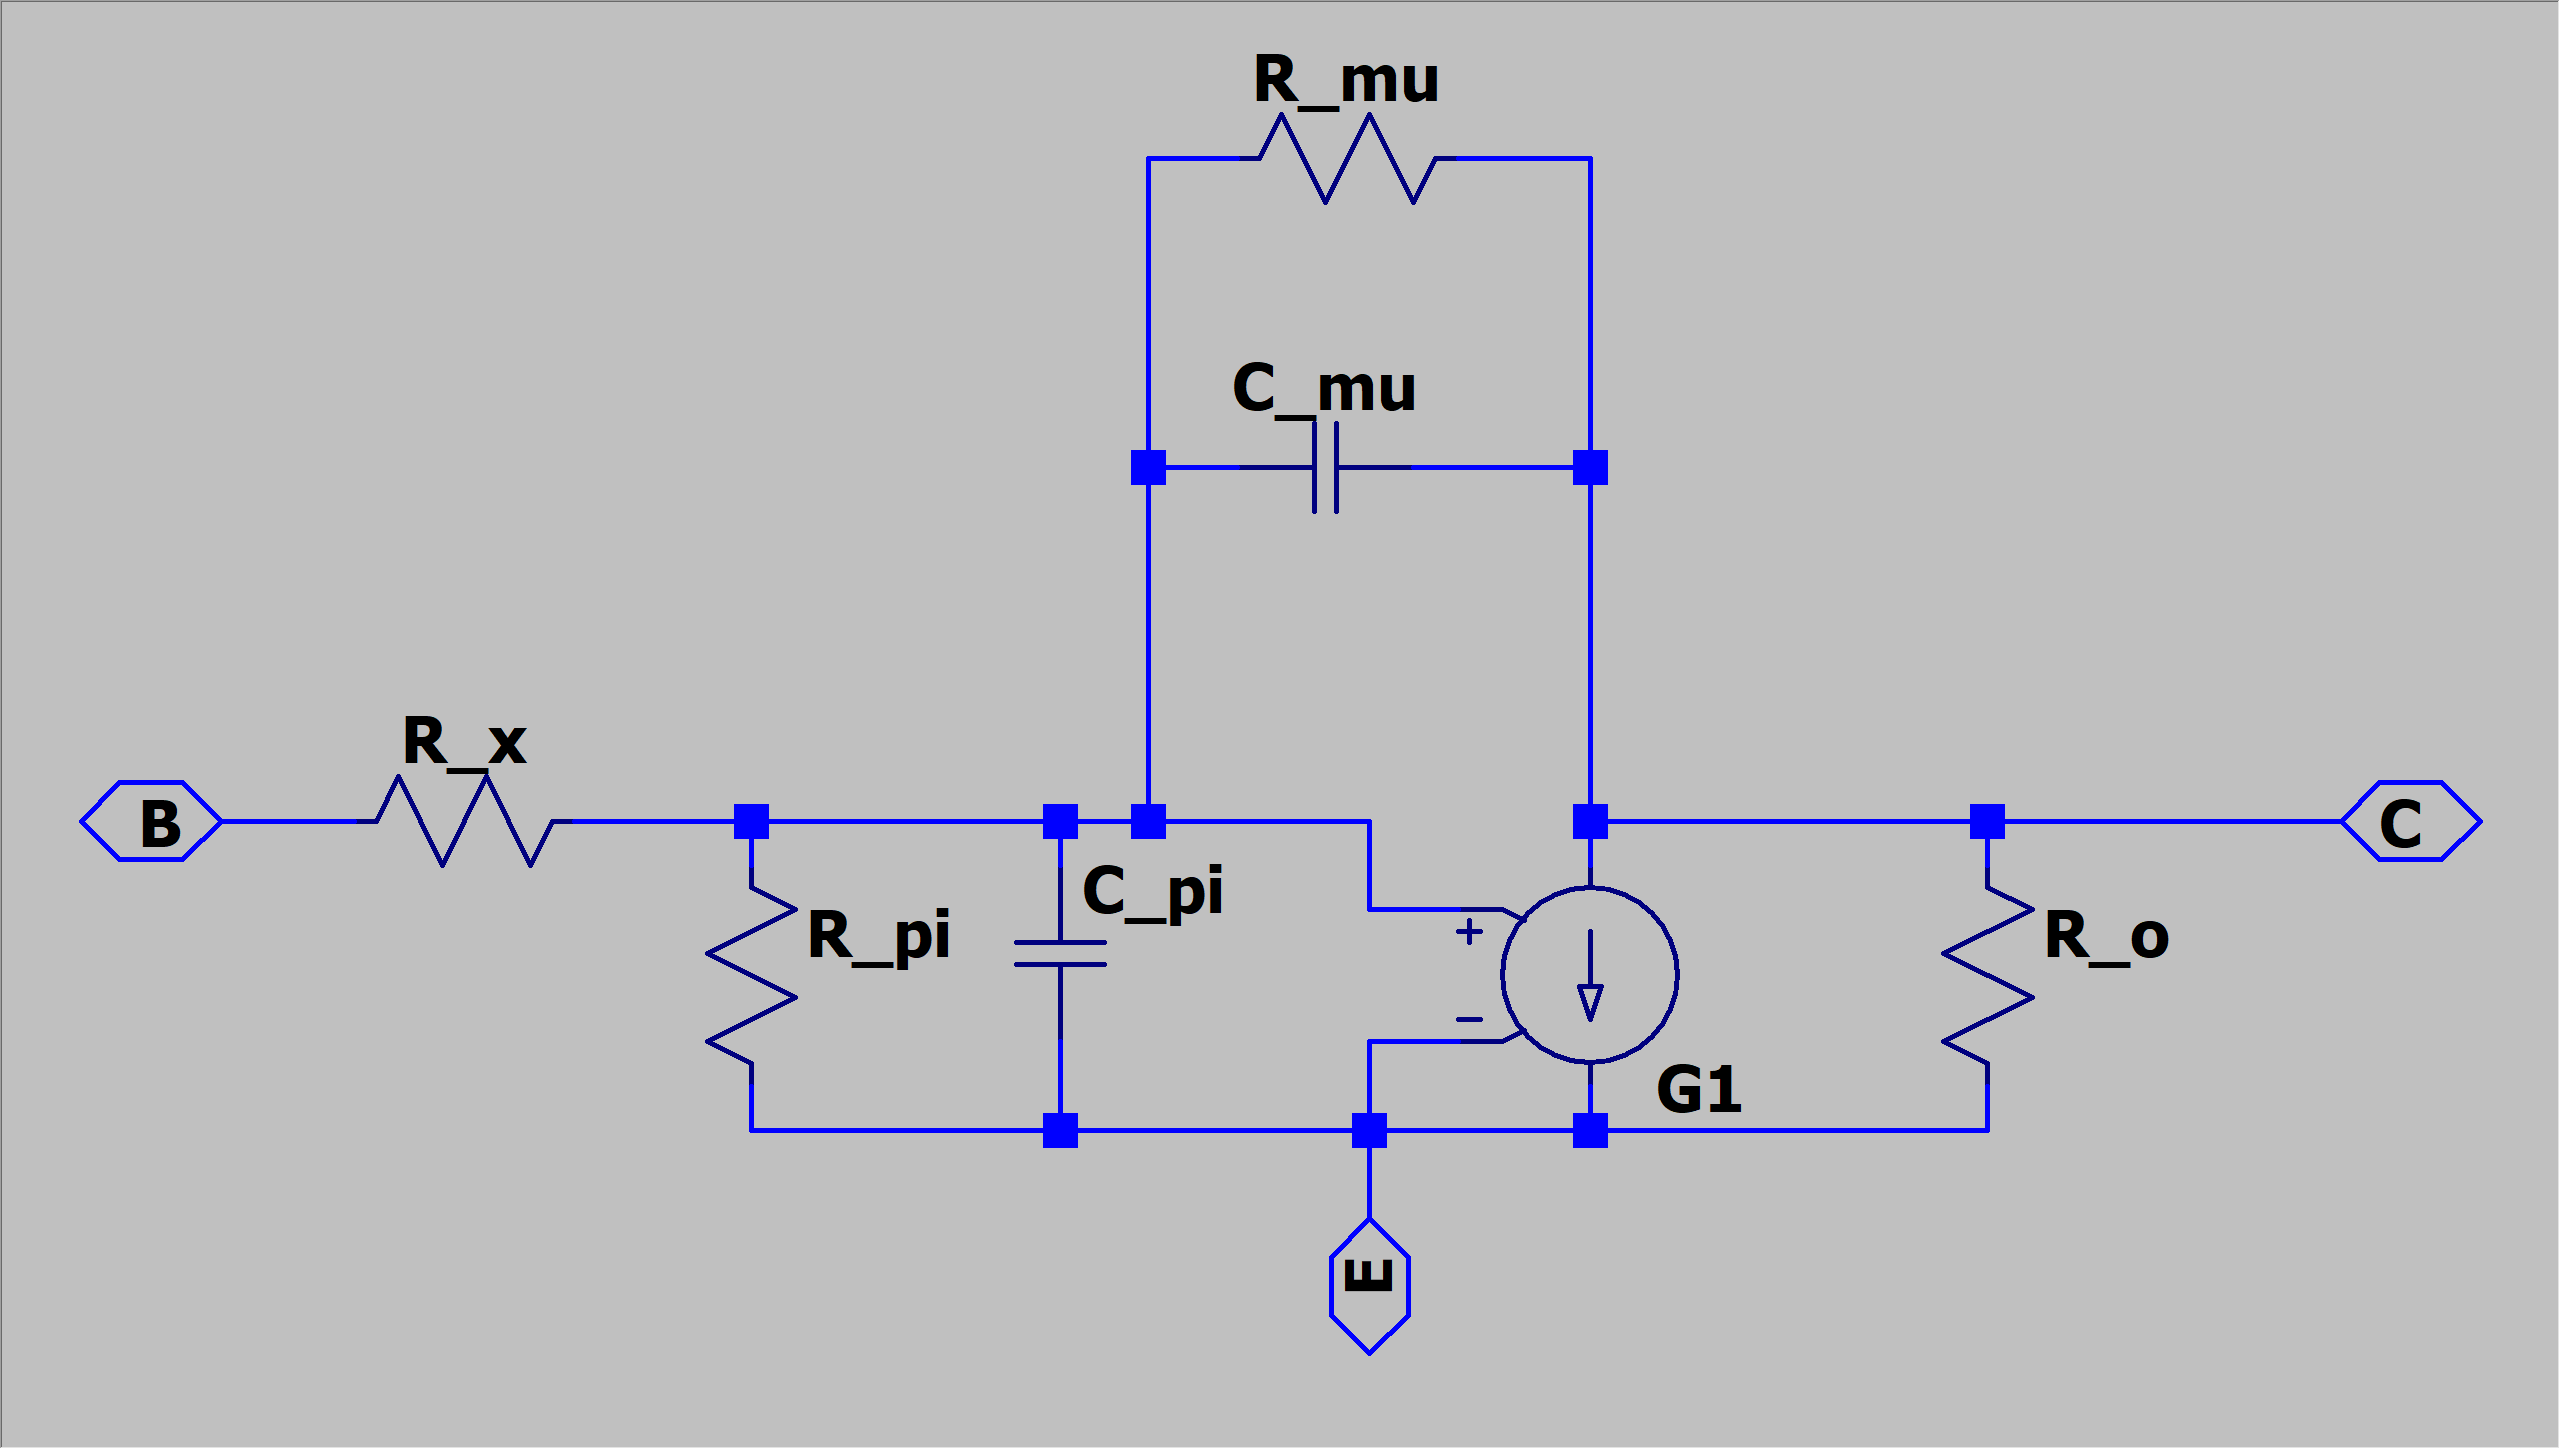
\includegraphics[width=0.4\textwidth]{figures/LTSpice-H-pi.png}}
    \caption{Hybrid-$\pi$ model in LTSpice}
    \label{fig:LTSpice-H-pi}
\end{figure}

\section{Analysis}

\subsection{LTSpice Models}

We used SPICE (Simulation Program with Integrated Circuit Emphasis) software to run our simulations, specifically the LTSpice
distribution by Analog Devices. The simulation setup in LTSpice consists of graphically laying out a circuit, assigning values
to the components, configuring simulation parameters, and running the simulation. fig. \ref{fig:LTSpice-H-pi} shows the
hybrid-$\pi$ model from fig. \ref{fig:hybrid-pi-model} set up in LTSpice. This model is not quite complete enough to run a 
simulation since the values of each component has not been assigned yet and there are no power and signal related components.

\subsubsection{Hybrid-$\pi$ model parameters}

\begin{table}[htbp]
    \centering
    \caption{Calculated parameters for hybrid-$\pi$ models}
    \begin{tabular}{|c|c|c|c|}
        \hline
        Parameter & Si & InGaP & Unit\\
        \hline
        $g_m$ & $3.894 \times 10^{-2}$ & $1.073 \times 10^{-2}$ & $\mho$ \\
        $r_x$ & 580 & 53 & $\Omega$ \\
        $r_\pi$ & 6420 & 2609 & $\Omega$ \\
        $c_\pi$ & $1.666 \times 10^{-11}$ & $1.148 \times 10^{-14}$ & F \\
        $r_\mu$ & $15.12 \times 10^{6}$ & 11.01 & $\Omega$ \\
        $c_\mu$ & $4 \times 10^{-12}$ & $3.5 \times 10^{-15}$ & F \\
        $r_0$ & $2.522 \times 10^{5}$ & 10.93 & $\Omega$ \\
        \hline
    \end{tabular}
    \label{tab:h-pi_params}
\end{table}

To determine the values for each component we used calculations outlined by Malik \cite{Malik1990} and Ramanan
\cite{ramanan_functional_1985} with a combination of transistor h-parameters provided by manufacturer datasheets
for the 2N3904 \cite{3904}, and transistor t-parameters found in literature for the InGaP HBT\cite{Oka2001}.
Table \ref{tab:h-pi_params} lists the parameters that were calculated for the Si and InGaP hybrid-$\pi$ model. Worked out
calculations for these parameters are given in Appendixes \ref{appendix-Si} and \ref{appendix-InGaP}

\subsubsection{Simple Amplifier Circuits}

\begin{figure}[htbp]
    \centering
    \begin{subfigure}[b]{0.45\textwidth}
        \centerline{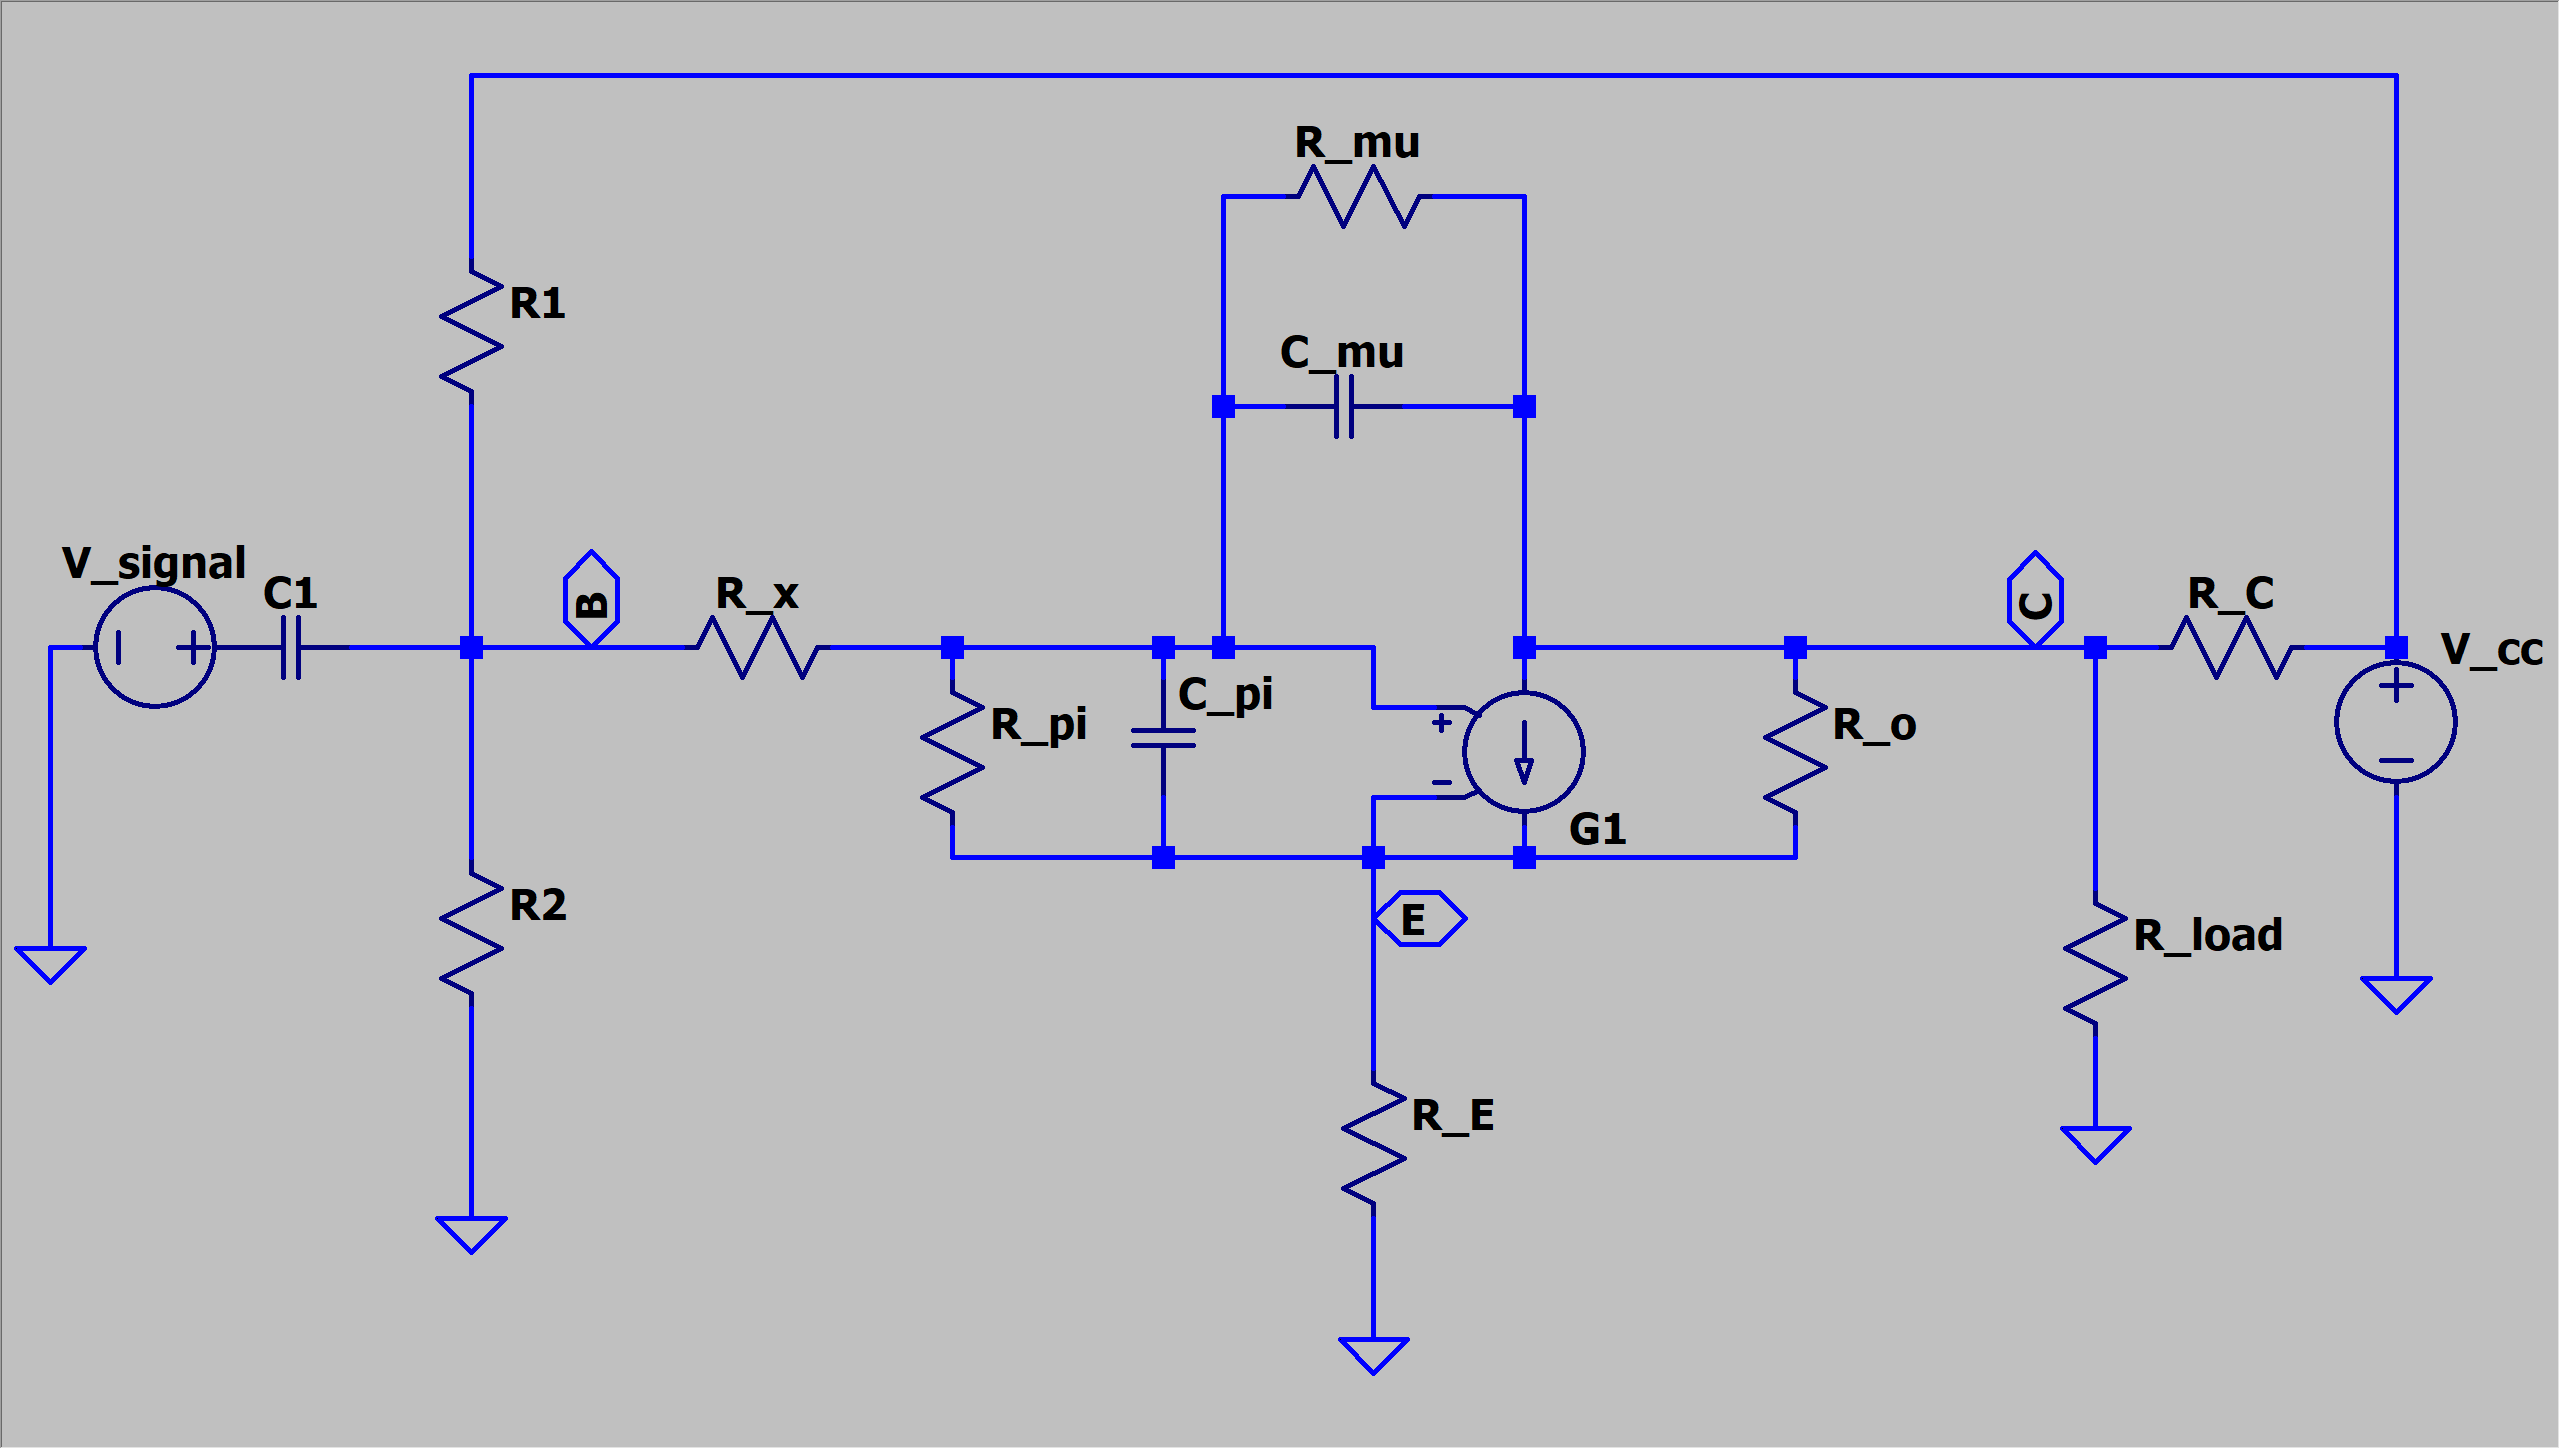
\includegraphics[width=\textwidth]{figures/LTSpice-CE.png}}
        \caption{Common Emitter}
        \label{fig:LTSpice-CE-fig}
    \end{subfigure}
    \par\bigskip
    \begin{subfigure}[b]{0.45\textwidth}
        \centerline{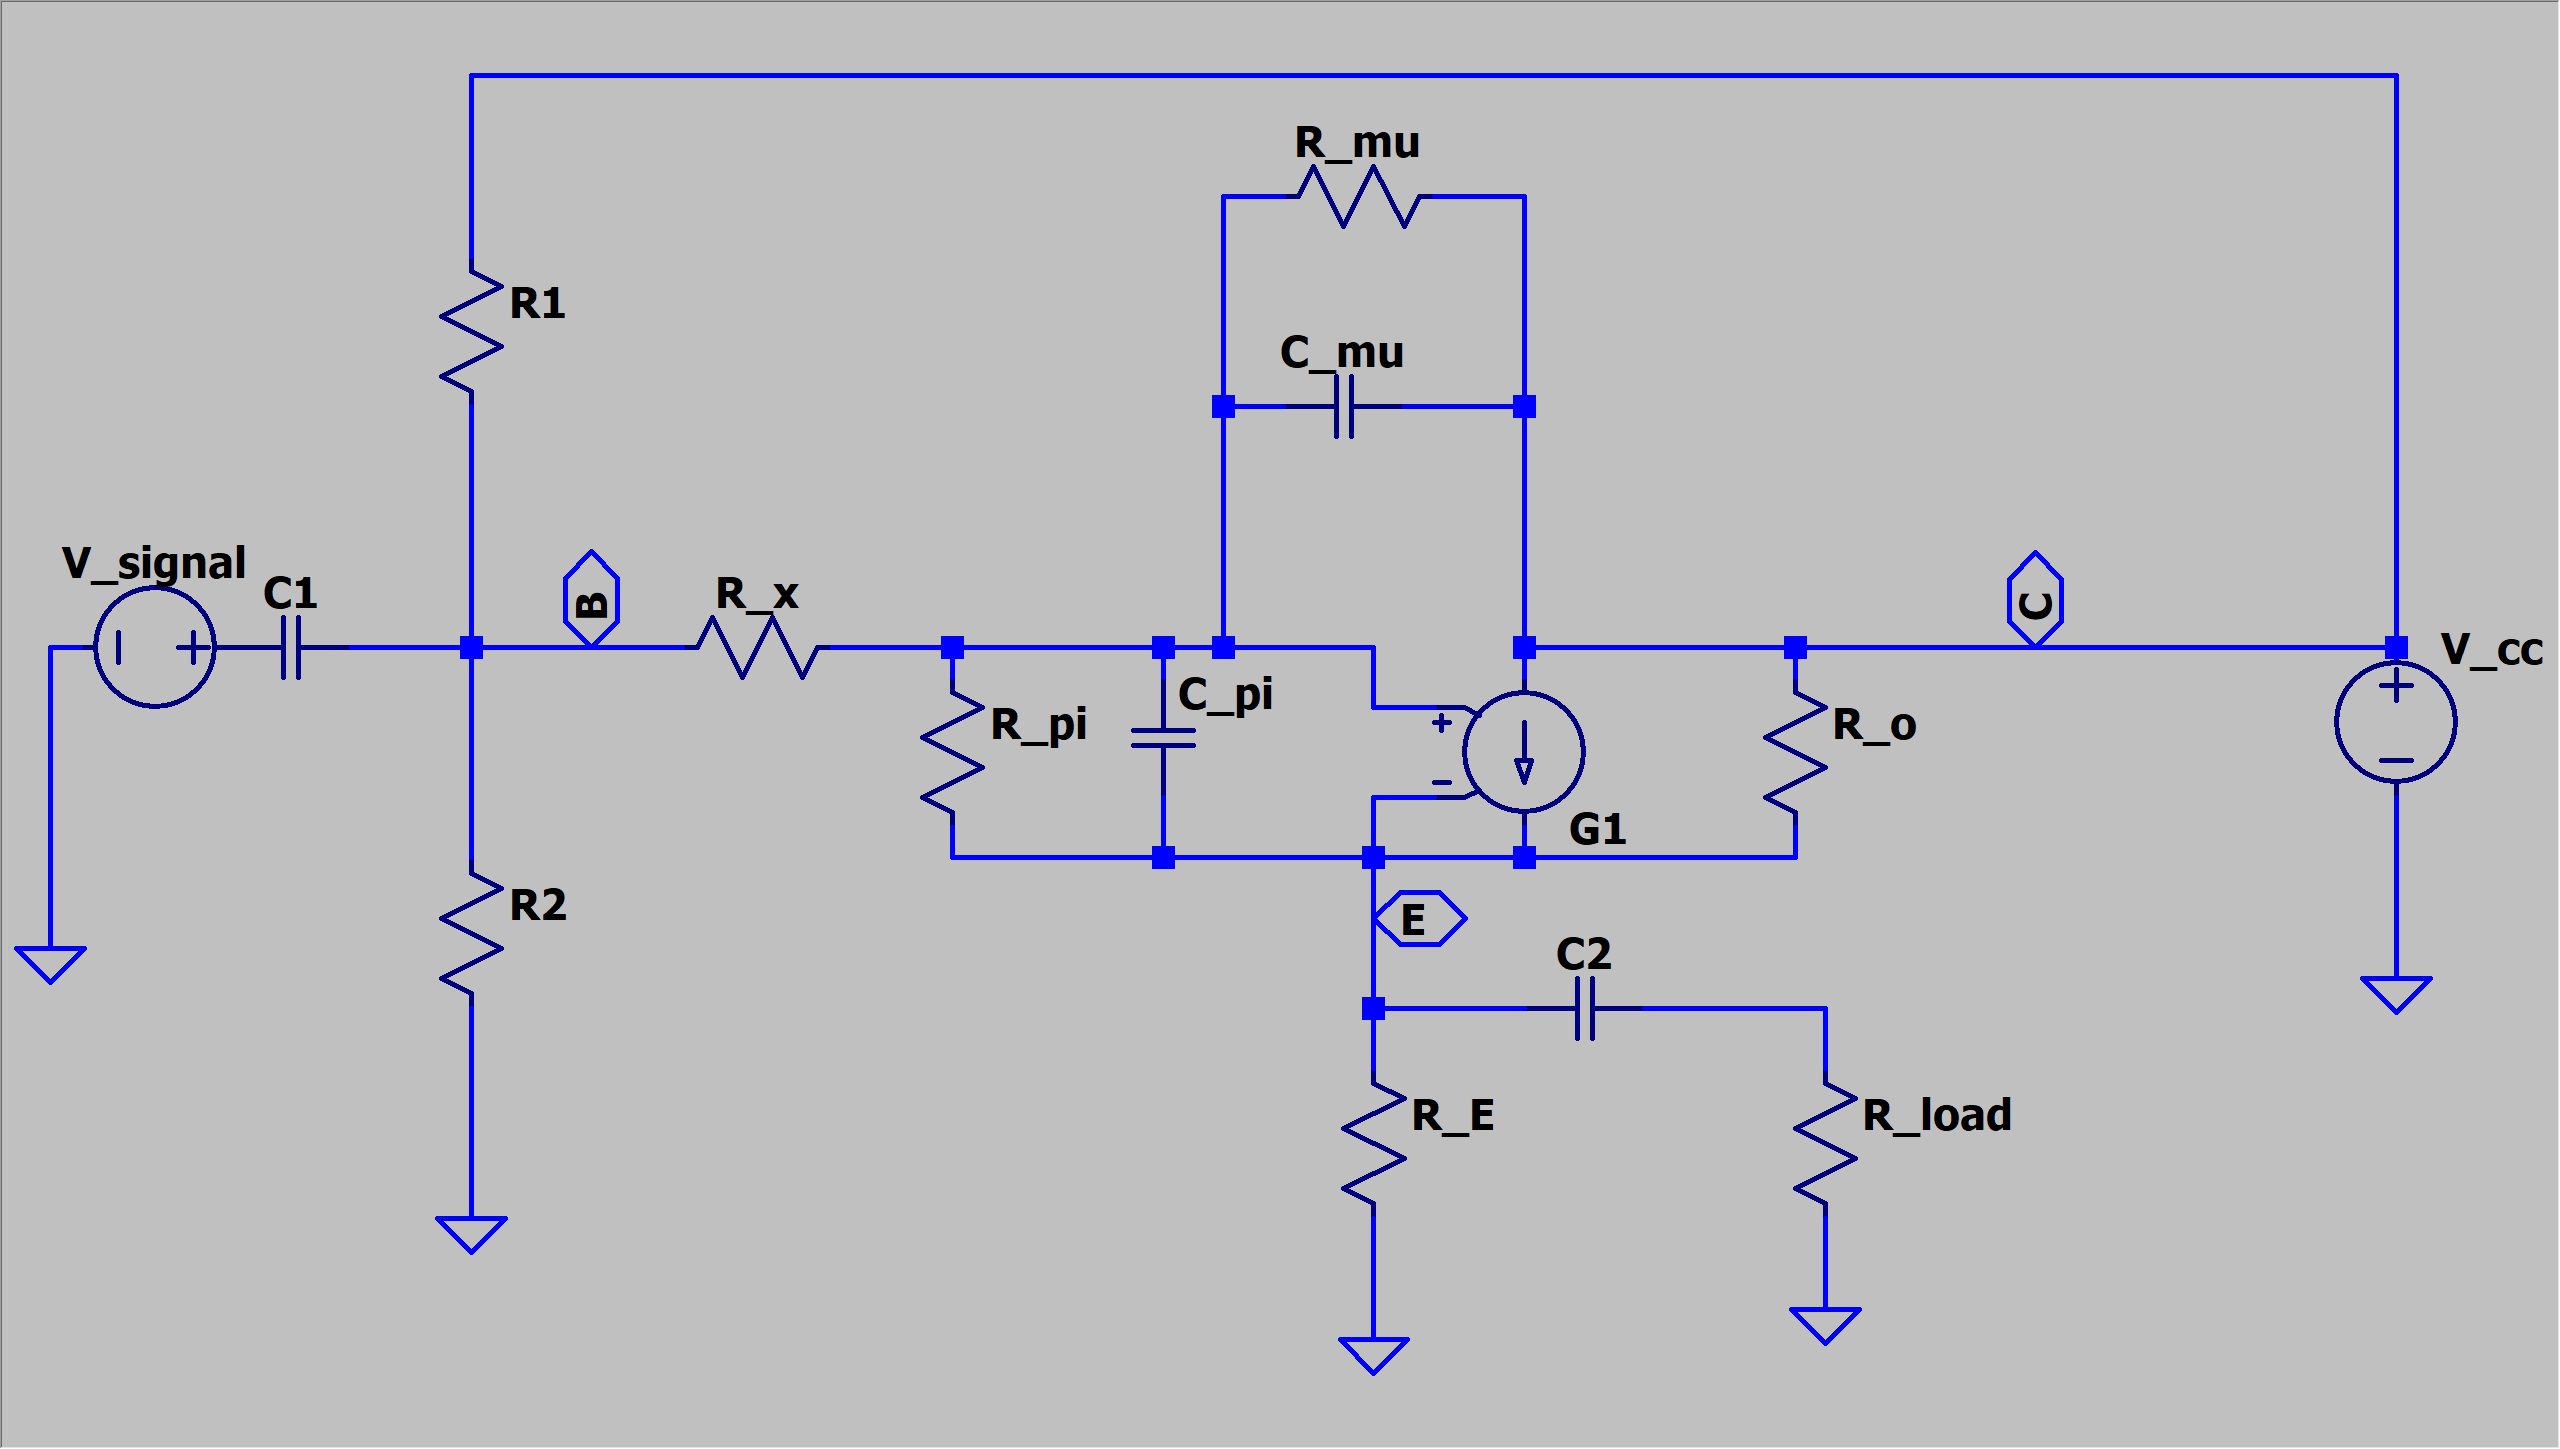
\includegraphics[width=\textwidth]{figures/LTSpice-CC.png}}
        \caption{Common Collector}
        \label{fig:LTSpice-CC-fig}
    \end{subfigure}
    \caption{Simple NPN amplifier circuits in LTSpice}
\end{figure}

\begin{figure*}[htbp]
    \centering
    \begin{subfigure}[b]{\textwidth}
        \centerline{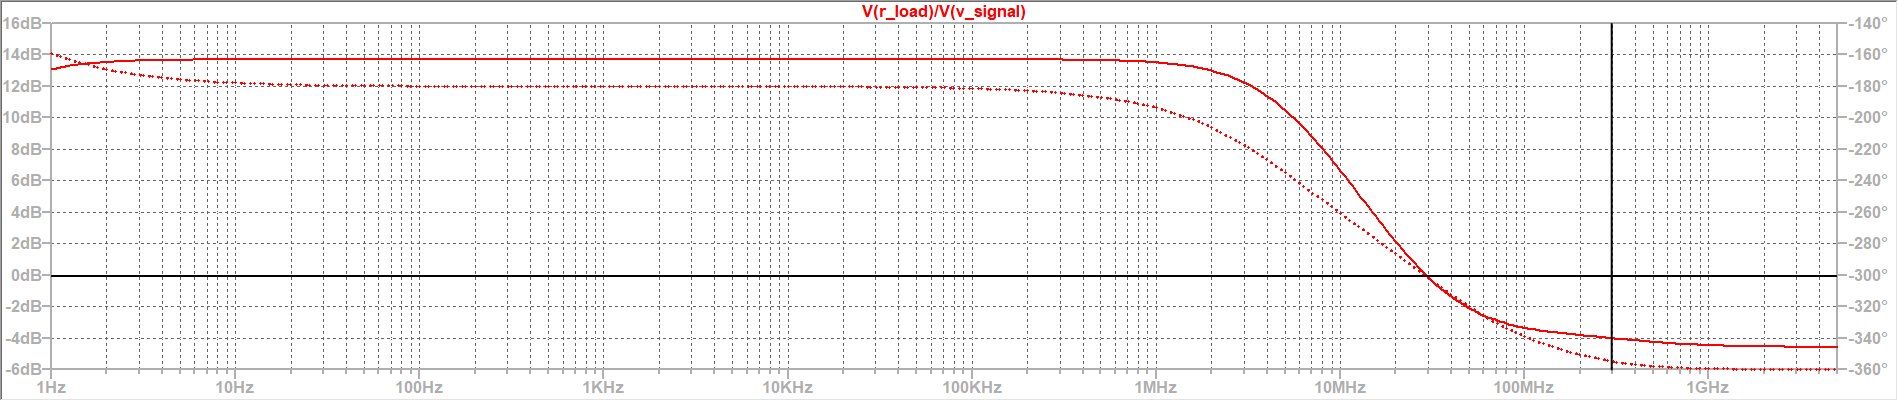
\includegraphics[width=\textwidth]{figures/Si-Result-CE.png}}
        \caption{Common Emitter Amplifier Results for Silicon. The vertical axis represents the voltage gain}
        \label{fig:Si-Result-CE}
    \end{subfigure}
    \par\bigskip
    \begin{subfigure}[b]{\textwidth}
        \centerline{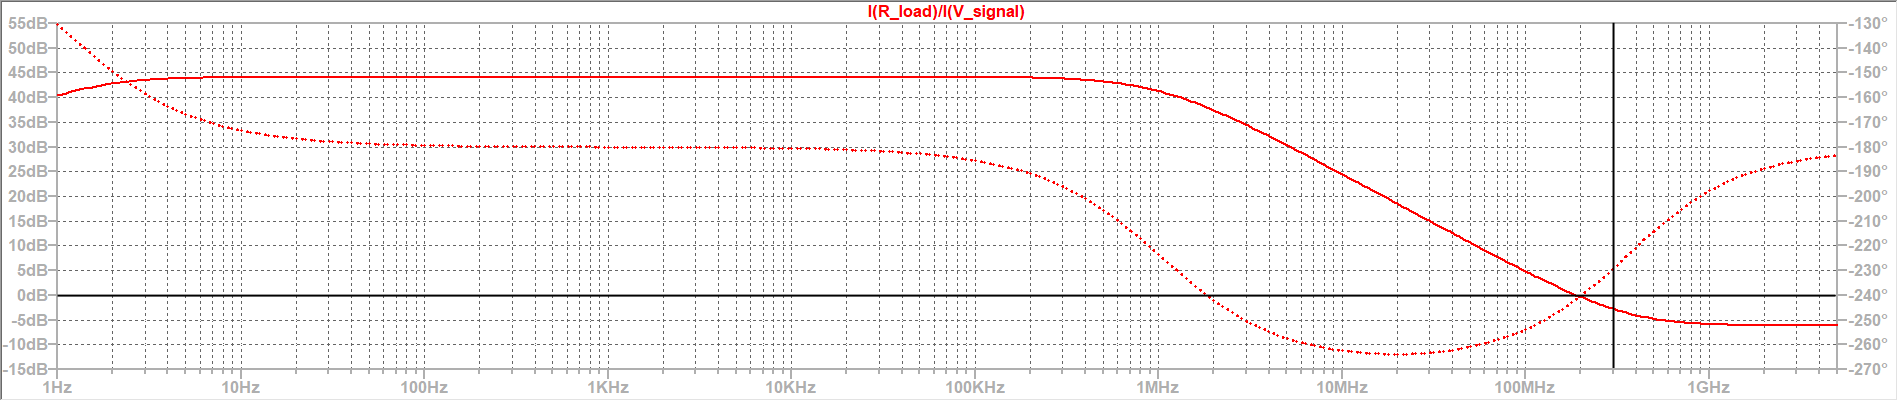
\includegraphics[width=\textwidth]{figures/Si-Result-CC.png}}
        \caption{Common Collector Amplifier Results for Silicon. The vertical axis represents the current gain}
        \label{fig:Si-Result-CC}
    \end{subfigure}
    \caption{Simple Amplifier Circuit Results for Silicon. The Vertical axis is the relative gain between the input signal and output load.
        The horizontal axis is the frequency. The bold black lines represent the 0 dB gain line in the vertical and the specified unity gain
        point in the horizontal.}
\end{figure*}

Before we could use these parameters in the full test circuits, fig. \ref{fig:ERA-50SM} and \ref{fig:ERA-Test-circuit}, we ran the
BJT/HBT models in simple amplifier circuits to ensure that they exhibit expected behavior. For this testing we are using common collector
ans common emitter amplifier circuits, fig. \ref{fig:NPN-CC-fig} and \ref{fig:NPN-CE-fig} from above. We then transferred the schematics
into LTSpice, fig. \ref{fig:LTSpice-CE-fig} and \ref{fig:LTSpice-CC-fig}, and determined the values for the external resistors, capacitors,
and voltage sources. The parameters for the external were calculated from Horowitz \cite{horowitz_art_2015}. For $V_{cc} = 10 V$ the external capacitor
and resistor values were: $R_1 = 88 k\Omega, R_2 = 110 k\Omega, R_E = 5 k\Omega, R_{Load} = 50 \Omega, C_1 = 47 \mu F, C_2 = 470 \mu F$.
For our first simulation run we set the $V_{signal}$ AC input to have an amplitude $0.1V$, a sufficiently low amplitude to stay within a small signal
model. We then ran an sinusoidal AC sweep between 1 Hz and 5 GHz ($5 \times 10^9$ Hz) to verify that we were seeing positive current/voltage gains
and that the unity gain frequencies, where the gain should be 0 dB, is close to the frequencies specified in the literature or datasheets.

\section{Results}

\subsection{Common Emitter and Common Collector Amplifier Simulations}

The silicon common emitter and common collector amplifier AC sweep results are shown in fig. \ref{fig:Si-Result-CE} and \ref{fig:Si-Result-CC}.
The results looked very promising at first. The common collector simulation had good level of gain and slowly ramped down to the unity gain
which was close to the specified value of 300 MHz. The common emitter simulation also showed decent levels of gain but missed the unity
gain mark by an order of magnitude. The silicon simulation results came out promising so we proceeded to the InGaP simulation.

The InGaP common collector and common emitter simulation results are shown in fig. \ref{fig:InGaP-Result-CE} and \ref{fig:InGaP-Result-CC}.
Unfortunately the results for this set of simulations was much less promising. We tried modifying the external component values, the input
signal amplitude but we still ended up with negative gains, or attenuations, in our InGaP simulation. Since this model should be showing at least
a positive gain we ran additional simulations to determine if our model was adequate for the simulations we are planning to run.

\begin{figure*}[htbp]
    \centering
    \begin{subfigure}[b]{\textwidth}
        \centerline{\includegraphics[width=\textwidth]{figures/InGaP-Result-CE.png}}
        \caption{Common Emitter Amplifier Results for InGaP. The vertical axis represents the voltage gain}
        \label{fig:InGaP-Result-CE}
    \end{subfigure}
    \par\bigskip
    \begin{subfigure}[b]{\textwidth}
        \centerline{\includegraphics[width=\textwidth]{figures/InGaP-Result-CC.png}}
        \caption{Common Collector Amplifier Results for InGaP. The vertical axis represents the current gain}
        \label{fig:InGaP-Result-CC}
    \end{subfigure}
    \caption{Simple Amplifier Circuit Results for Silicon. The Vertical axis is the relative gain between the input signal and output load.
        The horizontal axis is the frequency. As you can see both gains are in the negative region.}
\end{figure*}

\subsubsection{DC Analysis}

For our additional test to verify our model we chose to run some basic DC analysis simulations, specifically an analysis to characterize the
current-voltage curve of the transistor model. For our InGaP model we expect the curve to resemble that of fig. \ref{fig:InGaP-IV}. fig.
\ref{fig:InGaP-IV} shows the current at the collector, $I_C$, relative to the voltage between the collector and emitter, $V_{CE}$, of the
junction transistor. The several curves represents increasing input currents at the base, $I_B$, of the transistor in 10 $\mu A$ steps. This plot
shows that at very low collector-emitter voltages there is very little current gain but as the voltage increases the gain between the current
at the base and collector increases until a certain voltage, called the saturation voltage, where the collector current stays relatively constant
with increasing collector-emitter voltage. This type of behavior is exhibited by all junction based transistors \cite{sze_physics_2007}.

\begin{figure}[hbt!]
    \centerline{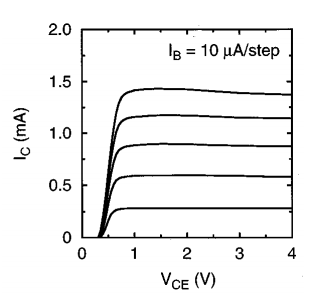
\includegraphics[width=0.25\textwidth]{figures/InGaP-IV.png}}
    \caption{The characteristic current-voltage curve of an InGaP HBT transistor. Notice how the collector current $I_C$ plateaus after around 0.5 - 0.6
    $V_{CE}$. \\ Source: \cite{Oka2001}}
    \label{fig:InGaP-IV}
\end{figure}

When we ran a DC analysis on the InGaP model to characterize it's current-voltage curve were given the result seen in fig. \ref{fig:InGaP-LT-IV}.
We can see that the model does show a steady rise in the collector current, $I_C$ plotted on the vertical axis, as the collector emitter voltage increases.
Where this model fell short is that there is no transition, at a saturation voltage, from the steady increase in the collector current to a plateau in the
collector current. From this result the hybrid-$\pi$ model seems to be inadequate for the series of tests we had planned to carry out.

\begin{figure}[hbt!]
    \centerline{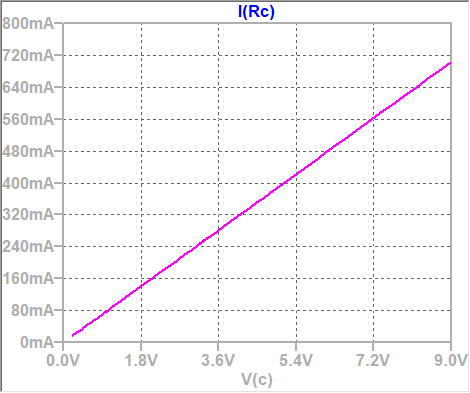
\includegraphics[width=0.3\textwidth]{figures/InGaP-LT-IV.png}}
    \caption{DC simulation of the hybrid-$\pi$ InGaP model does not follow the plateau that is to be expected with an junction transistor}
    \label{fig:InGaP-LT-IV}
\end{figure}

\section{Conclusion}

Even though we were not able to reach a consensus on the performance of Silicon and InGaP junction transistors we were able to discover shortcomings in
the popular hybrid-$\pi$ equivalent circuit transistor model and paved the groundwork for future research with models that more accurately predict the
behavior of junction transistors.

\subsection{Limitations}

The biggest limitation that we had in this project was our choice of using the hybrid-$\pi$ model for our simulations. This model works on the assumption
that the junction transistor is purely a current amplifier device. In reality a junction transistor can be used as a current amplification device, but more
importantly, it is a device constructed from a pair of junctions between positively and negatively doped semiconductor material \cite{sze_physics_2007}.
This gives it properties such as the current-voltage curve and saturation voltage we saw from from fig. \ref{fig:InGaP-IV}. With this limitation we were
not able to simulate the circuits we originally planned. Another limitation that we had in this project is that we only chose to model a single type of
silicon BJT rather than sample a wide range to pick one that could possibly perform the best at ultra high frequencies. We were also limited in this project
by the fact that we were not able to find a specific InGaP HBT part that had a nicely formatted datasheet and specifications we could calculate our parameters
with. Instead we had to rely on research literature where the data was not as centralized. This meant that the data that we gathered may not be a very fair
comparison with InGaP HBTs in general or match very closely with the InGaP HBTs inside the ERA-50SM+ device.

\subsection{Future Work}

Some possible paths that could be taken for future work include developing a better simulation model to more accurately model the behavior of a junction
transistor, taking a wider sample of silicon BJTs to find more ultra high speed optimized types, and doing deeper research into InGaP HBTs to come up with
a better set of parameters. Developing a better simulation model for junction transistors will increase the accuracy of our results to the real world
behavior of junction transistors. Simulating a broader range of silicon transistors and digging deeper into InGaP transistor parameters will provide fairer
comparison between the two materials.

\appendices

\setcounter{table}{0}
\renewcommand{\thetable}{A\arabic{table}}

\section{Calculations for Silicon Hybrid-$\pi$ Model}
\label{appendix-Si}

Table \ref{tab:kec-3904} shows the data we gathered for the 2N3904 Silicon BJT parameters from KEC Semiconductor \cite{3904}.

\begin{table}[htbp]
    \centering
    \caption{Data gathered from KEC 3904 datasheet \\ Compiled from \cite{3904}}
    \begin{tabular}{|c|c|c|c|}
        \hline
        Parameter & Value\\
        \hline
        $f_T$ & $300 \times 10^6$ Hz \\
        Unity Gain Frequency & \\
        \hline
        $I_C$ & 10V \\
        Collector Current at h-parameter test condition & \\
        \hline
        $h_{ie}$ & $7 \times 10^{3} \Omega$ \\
        Input Impedance & \\
        \hline
        $h_{re}$ & $4.25 \times 10^{-4}$ \\
        Voltage Feedback Ratio & \\
        \hline
        $beta = h_{fe}$ & 250 \\
        Small-Signal Current Gain & \\
        \hline
        $h_{oe}$ & $20.5 \times 10^{-6} \mho$ \\
        Collector Output Admittance & \\
        \hline
        $C_{ob} = C_{\mu}$ & $4 \times 10^{-12}$ F \\
        Collector Output Capacitance & \\
        \hline
    \end{tabular}
    \label{tab:kec-3904}
\end{table}

The following calculations use equations collected from \cite{Malik1990}.

To calculate the transconductance, $g_m$, we need the collector current at the h-parameter test condition, $I_C$, and the thermal
voltage, $V_T$.

\begin{equation}
    \begin{aligned}
        V_T &= \frac{kT}{q} \\
        V_T &= \frac{1.38 \times 10^{-28} \times 298.15}{1.602 \times 10^{-19}} \\
        V_T &= 0.02568V = 25.68 mV
    \end{aligned}
\end{equation}

where k is the Boltzmann Constant, T is the temperature in kelvin, and q is the charge of an electron

\begin{equation}
    \begin{aligned}
        g_m &= \frac{I_C}{V_T} \\
        g_m &= \frac{1 \times 10^{-3}}{0.02568} \\
        g_m &= 0.03894
    \end{aligned}
\end{equation}

To calculate the input resistance, $r_\pi$, we need the transconductance, $g_m$, and the small-signal current gain, $\beta = h_{fe}$.

\begin{equation}
    \begin{aligned}
        r_{\pi} &= \frac{\beta}{g_m} \\
        r_{\pi} &= \frac{250}{0.03894} \\
        r_{\pi} &= 6420
    \end{aligned}
\end{equation}

To calculate the feedback resistance, $r_{\mu}$, we need the input resistance, $r_{\pi}$, and the voltage feedback ratio, $h_{re}$.

\begin{equation}
    \begin{aligned}
        r_{\mu} &= \frac{r_{\pi}}{h_{re}} \\
        r_{\mu} &= \frac{6420}{4.25 \times 10^{-4}} \\
        r_{\mu} &= 15.12 \times 10^6
    \end{aligned}
\end{equation}

To calculate the output resistance, $r_0$, we need the collector output admittance, $h_{oe}$, small-signal current gain, $\beta = h_{fe}$,
and the feedback resistance, $r_{\mu}$.

\begin{equation}
    \begin{aligned}
        r_0 &= \left(h_{oe} - \frac{\beta}{r_{\mu}} \right)^{-1} \\
        r_0 &= \left(20.5 \times 10^{-6} - \frac{250}{15.12 \times 10^6} \right)^{-1} \\
        r_0 &= 2.522 \times 10^5
    \end{aligned}
\end{equation}

To calculate the spreading resistance, $r_x$, we need the input impedance, $h_{ie}$, and the input resistance, $r_{\pi}$.

\begin{equation}
    \begin{aligned}
        r_x &= h_{ie} - r_{\pi} \\
        r_x &= 7 \times 10^3 - 6420 \\
        r_x &= 580
    \end{aligned}
\end{equation}

To interelectrode capacitance, $c_{\pi}$, we need the transconductance, $g_m$, the unity gain frequency, $f_T$, and the
Collector Output Capacitance, $c_{\mu}$.

\begin{equation}
    \begin{aligned}
        c_{\pi} &= \frac{g_m}{2 \pi f_T} - c_{\mu} \\
        c_{\pi} &= \frac{0.03894}{2 \pi 300 \times 10^6} - 4 \times 10^{-12} \\
        c_{\pi} &= 1.666 \times 10^{-11}
    \end{aligned}
\end{equation}



\section{Calculations for InGaP Hybrid-$\pi$ Model}
\label{appendix-InGaP}

Table \ref{tab:InGaP-Params} shows the data we gathered for the InGaP parameters from T. Oka et al. \cite{Oka2001}.

\begin{table}[htbp]
    \centering
    \caption{Data gathered from T. Oka et al. \\ Compiled from \cite{Oka2001}}
    \begin{tabular}{|c|c|c|c|}
        \hline
        Parameter & Value\\
        \hline
        $f_T$ & $114 \times 10^9$ Hz \\
        Unity Gain Frequency & \\
        \hline
        $h_{fe}$ & 28 \\
        Small-Signal Current Gain & \\
        \hline
        $r_e$ & $90 \Omega$ \\
        Emitter Resistance & \\
        \hline
        $r_b = r_x$ & $53 \Omega$ \\
        Base Resistance & \\
        \hline
        $r_c$ & $11 \Omega$ \\
        Collector Resistance & \\
        \hline
        $C_{\mu}$ & $3.5 \times 10^{-15}$ F \\
        Collector Capacitance & \\
        \hline
    \end{tabular}
    \label{tab:InGaP-Params}
\end{table}

Since the parameter we gathered are in t-parameter format we have to first convert them to h-parameters then to the values for
a hybrid-$\pi$ model

The following calculations use equations collected from Ramanan \cite{ramanan_functional_1985}.

To find our t-parameter $\alpha$ value we need the small signal current gain, $h_{fe}$.

\begin{equation}
    \begin{aligned}
        h_{fe} &= \frac{\alpha}{1 - \alpha} \\
        28 &= \frac{\alpha}{1 - \alpha} \\
        28 (1 - \alpha) &= \alpha \\
        28 &= 29 \alpha \\
        \alpha &= 0.9665
    \end{aligned}
\end{equation}

To find the input impedance, $h_{ie}$, we need the $\alpha$ value, the emitter resistance, $r_e$, and the base
resistance $r_b$.

\begin{equation}
    \begin{aligned}
        h_{ie} &= \frac{r_e}{1 - \alpha} + r_b \\
        h_{ie} &= \frac{90}{1 - 0.9655} + 53 \\
        h_{ie} &= 2662
    \end{aligned}
\end{equation}

To find the voltage feedback ratio, $h_{re}$, we need the $\alpha$ value, the emitter resistance, $r_e$, and the
collector resistance, $r_c$.

\begin{equation}
    \begin{aligned}
        h_{re} &= \frac{r_e}{\left(1 - \alpha\right) r_c} \\
        h_{re} &= \frac{90}{\left(1 - 0.9655\right) 11} \\
        h_{re} &= 237
    \end{aligned}
\end{equation}

To find the collector output admittance, $h_{oe}$, we need the $\alpha$ value and the collector resistance $r_c$

\begin{equation}
    \begin{aligned}
        h_{oe} &= \frac{1}{\left(1 - \alpha \right) r_c} \\
        h_{oe} &= \frac{1}{\left(1 - 0.9655\right) 11}
        h_{oe} &= 2.635
    \end{aligned}
\end{equation}

To find the transconductance, $g_m$, we need the small-signal current gain, $h_{fe}$, the input impedance, $h_{ie}$,
and the base resistance, $r_b = r_x$.

\begin{equation}
    \begin{aligned}
        g_m &= \frac{h_{fe}}{h_{ie} - rx} \\
        g_m &= \frac{28}{2662 - 53} \\
        g_m &= 0.01073
    \end{aligned}
\end{equation}

To calculate the input resistance, $r_\pi$, we need the input impedance, $h_{ie}$, and the base resistance, $r_b = r_x$.

\begin{equation}
    \begin{aligned}
        r_{\pi} &= h_{ie} - r_x \\
        r_{\pi} &= 2662 - 53 \\
        r_{\pi} &= 2609
    \end{aligned}
\end{equation}

To calculate the feedback resistance, $r_{\mu}$, we need the input impedance, $h_{ie}$, the base resistance, $r_b = r_x$, and
the voltage feedback ratio, $h_{re}$.

\begin{equation}
    \begin{aligned}
        r_{\mu} &= \frac{h_{ie} - r_x}{h_{re}} \\
        r_{\mu} &= \frac{2662 - 53}{237} \\
        r_{\mu} &= 11.01
    \end{aligned}
\end{equation}

To calculate the output resistance, $r_0$, we need the collector output admittance, $h_{oe}$, small-signal current gain, $h_{fe}$,
the input impedance, $h_{ie}$, the voltage feedback ratio, $h_{re}$, and the base resistance, $r_b = r_x$.

\begin{equation}
    \begin{aligned}
        r_0 &= \left(h_{oe} - \frac{h_{fe} h_{re}}{h_{ie} - r_x}\right)^{-1} \\
        r_0 &= \left(2.635 - \frac{(28)(237)}{2662 - 53}\right)^{-1} \\
        r_0 &= 10.93
    \end{aligned}
\end{equation}

\section*{Acknowledgment}

The author would like to thank Dr. S. Ramachandran for all the guidance and support for this project. The author would also like to thank
Dr. M. Gliboff and the UW Bothell physics class of 2021 for their support as well.

\bibliographystyle{IEEEtran}
\bibliography{bibliography}{}

\end{document}
